\section{Durchführung}

    Für die Messung werden zwei Laser verwendet,
    welche monochromatisches Licht der Wellenlänge $\lambda = \SI{635}{\nano\meter}$,
    also rotes Licht,
    und $\lambda = \SI{532}{\nano\meter}$,
    also grünes Licht erzeugen.
    \begin{figure}[H]
        \centering
        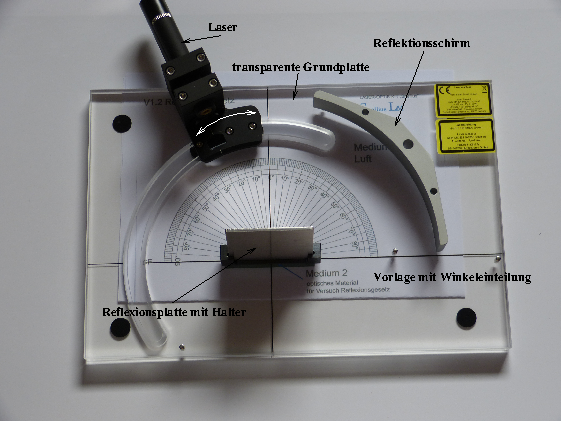
\includegraphics[scale=0.9]{content/img/Abb_3.pdf}
        \caption{Aufbau zur Untersuchung von Reflexion, Brechung und Beugung eines Lichtstrahls.}
        \label{fig:aufbau_platte}
    \end{figure}
    Die Laser sind auf einer transparenten Grundplatte befestigt,
    und lassen sich auf etwa einem Halbkreis um einen Punkt verschieben,
    auf dem verschiedene Objekte platziert werden können.
    Auf der transparenten Platte ist außerdem ein Reflexionsschirm angebracht,
    der auf zwei verschiedene Höhen eingestellt werden kann.
    Zur Messung wird die Platte auf eine Vorlage gestellt,
    welche eine Winkelunterteilung zeigt,
    auf dem die gemessenen Winkel abgelesen werden können.\\
    Dieser Aufbau ist in der Abbildung \ref{fig:aufbau_platte} gezeigt.\\
    Als optische Elemente dienen ein Spiegel,
    eine planparallele Platte sowie ein Prisma und Gitter verschiedener Gitterkonstanten.
    \begin{figure}[H]
        \centering
        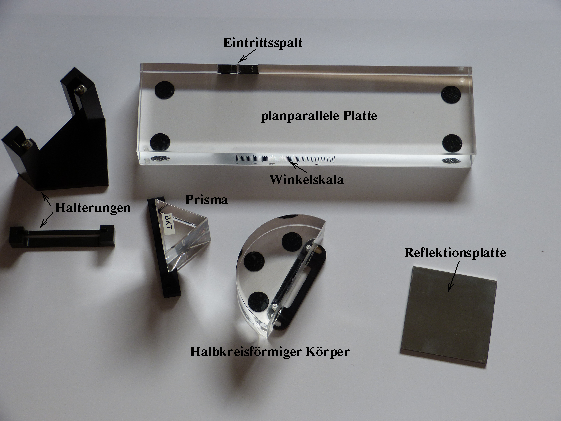
\includegraphics[scale=0.9]{content/img/Abb_4.pdf}
        \caption{Optische Elemente zur Messung von Reflexion, Brechung und Beugung.}
        \label{fig:aufbau_elemente}
    \end{figure}
    Das optisch dünnere Medium ist bei allen Versuchen Luft.

\subsection{Untersuchung der Reflexion}

    Für diese Messung wird der Spiegel in einer Halterung in die Mitte der transparenten Platte gestellt.
    Es wird die Vorlage A verwendet,
    sowie der grüne Laser.
    Nun wird der Laser verschoben,
    sodass der Lichtstrahl in einem Einfallswinkel $\alpha_1$ auf den Spiegel trifft.\\
    Es werden für sieben verschiedene Winkel $\alpha_1$ die Ausfallswinkel $\alpha_2$ gemessen.

\subsection{Untersuchung der Brechung}

    Diese Messung setzt sich aus zwei Teilen zusammen.
    Es wird einmal die Brechung an einer planparallelen Platte,
    sowie an einem Prisma untersucht.\\
    \\
    Für die Messung mit der planparallelen Platte werden der grüne Laser und die Vorlage A verwendet.
    Beim Aufstellen der planparallelen Platte,
    welche in Abbilung \ref{fig:aufbau_elemente} zu sehen ist,
    muss darauf geachtet werden,
    dass der Spalt auf der Platte zum Laser hin zeigt.
    Der Brechungswinkel kann mithilfe der Skala auf der anderen Seite abgelesen werden.\\
    Es werden für sieben verschiedene Einfallswinkel $\alpha$ die Brechungswinkel $\beta$ gemessen.\\
    \\
    Für die Messung der Brechung am Prisma werden beide Laser verwendet, 
    sowie die Vorlage,
    auf der ein Prisma-Umriss abgebildet ist.
    Das dreieckige Prisma wird in die Mitte der transparenten Platte gesetzt,
    wobei der Lichtstrahl auf eine der ebenen Flächen trifft.
    Gegenüber dem Laser wird eine Winkelskala aufgestellt,
    auf der auch die Lichtpunkte sichtbar gemacht werden.\\
    Es werden die Austrittswinkel $\alpha_2$ für sechs Einfallswinkel $\alpha_1$ gemessen,
    wobei $\alpha_1$ in einem Bereich von $\SI{10}{\degree} \leq \alpha_1 \leq \SI{60}{\degree}$ liegen soll.
    Diese Messung wird für beide Laser durchgeführt.

\subsection{Untersuchung der Beugung am Gitter}

    Für diese Messung wird ein Gitter vor der Kante der transparenten Platte platziert,
    damit beide Laserstrahlen durch das Gitter gelangen.
    Gegenüber der Laser wird eine Winkelskala von $\SI{-35}{\degree} \leq \varphi \leq \SI{35}{\degree}$ gestellt,
    auf der die Lichtpunkte,
    also die Intensitätsmaxima abgelesen werden können.\\
    Die Messung wird für beide Laser für die Gitter mit $\SI{600}{{Linien}\per\milli\meter}$,
    $\SI{300}{{Linien}\per\milli\meter}$ und $\SI{100}{{Linien}\per\milli\meter}$ durchgeführt,
    %TODO: Kann man das mit den Linienzahlen sonst noch schöner machen?
    wobei sich,
    abhängig von der Anzahl der Gitterlinien,
    verschieden viele Intensitätsmaxima ergeben.